%
% kont.tex -- slide template
%
% (c) 2021 Prof Dr Andreas Müller, OST Ostschweizer Fachhochschule
%
\bgroup
\begin{frame}[t]
\setlength{\abovedisplayskip}{5pt}
\setlength{\belowdisplayskip}{5pt}
\frametitle{Kontinuitätsgleichung}
\begin{center}
\begin{tikzpicture}[>=latex,thick]
\node at (0,0) {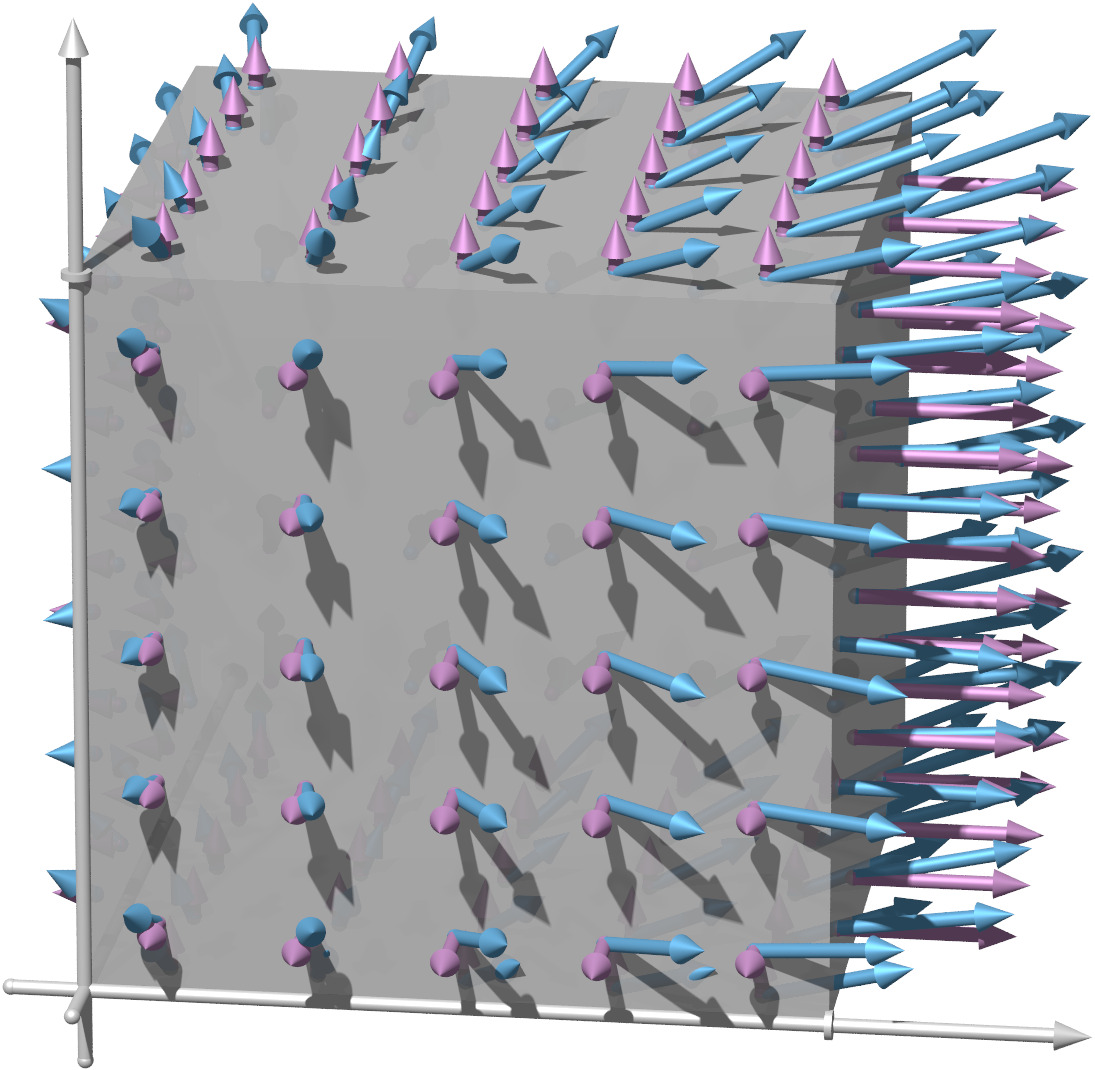
\includegraphics[width=7.1cm]{../slides/5/kont.jpg}};
\node at (1.9,-3.5) {$\Delta x$};
\node at (-2.3,3.3) {$\Delta y$};
\node at (-3.5,1.7) {$\Delta z$};
\node at (3.5,-3.0) {$x$};
\node at (-3.3,3.2) {$z$};
\end{tikzpicture}
\end{center}
\end{frame}
\egroup
